\chapter{Marco teórico}\label{ch:teoria}

\section{Ecuaciones y citar}\label{sec:ecuaciones}

\begin{comment}
  Objetivo: Explicarles a los lectores de computación que entienden
  los lingüistas de una variación dialectal
\end{comment}

El paquete cref permite citar de forma automática se reconozca si se trata de una tabla, ecuación, capítulo, o figura, empleando el comando \verb'\cref{}':

Ecuaciones de Navier-Stokes \cref{eq:NavierStokes,eq:continuty}.

En las \cref{fig:Cpx_rans_8,fig:Cpx_rans_10} , la  \cref{tab:dielectricK}... Para que la etiqueta de la referencia cruzada empiece con mayúsculas se usa \verb'\Cref{}': en el \Cref{c:codigo}, para minúsculas \verb'\cref{}': \cref{sec:ecuaciones}. 

Si se ha modificado el nombre de la etiqueta mediante \verb'\crefname{table}{Tabla}{Tablas}' aunque se use \verb'\cref{}' se imprimirá en mayúsculas: la \cref{tab:dielectricK}.

\begin{equation}\label{eq:continuty}
    \nabla\cdot \vec{u}
\end{equation}

\begin{equation}\label{eq:NavierStokes}
\frac{\partial \bar{u_i}}{\partial t} +\bar{u_j}\frac{\partial \bar{u_i}}{\partial x_j}=-\frac{1}{\rho}\frac{\partial \bar{p}}{\partial x_i}+\nu\frac{\partial^2 \bar{u_i}}{\partial x_j^2}+\frac{f_b}{\rho}
\end{equation}

Dividir una ecuación larga usando \verb'\dmath' del paquete breqn:

\begin{dmath}\label{eq:reynolds:_transport}
\frac{\partial}{\partial t}\left \langle u_i u_k\right \rangle+U_j\frac{\partial}{\partial x_j}\left \langle u_i u_j\right \rangle = \frac{p}{\rho}\left[\frac{\partial u_i}{\partial x_k}+\frac{\partial u_k}{\partial x_i} \right]+\frac{\partial}{\partial x_j}\left \{ -\frac{1}{\rho}\left[ \left \langle pu_k\right \rangle\delta_{ij}+\left \langle pu_i\right \rangle\delta_{kj}\right] -\left \langle u_i u_j u_k\right \rangle+ 2\nu\left [ s_{ij}u_k+s_{ikj}u_i \right ] \right \}-\left [ u_i u_j \frac{\partial U_k}{\partial x_j}+u_k u_j \frac{\partial U_i}{\partial x_j} \right ]-2\nu\left [ s_{ij} \frac{\partial u_k}{\partial x_j}+s_{kj}\frac{\partial u_i}{\partial x_j} \right ]
\end{dmath}

\subsection{Ecuaciones con physics}

Physics cuenta con comandos con los que es más fácil escribir expresiones como derivadas parciales', términos convectivos, etc. En el \href{http://mirrors.ibiblio.org/CTAN/macros/latex/contrib/physics/physics.pdf}{manual de usuario de Physics} se pueden consultar todos sus comandos.

\verb'\pdv{x}{t}': $\pdv{x}{t}$\\
\verb'\laplacian{x}': $\laplacian{x}$\\
\verb'\dv[n]{f}{x}': $\dv[n]{f}{x}$\\
\verb'\vb{x}': $\vb{x}$

\begin{equation}
    \div{\vb{u}}=0
\end{equation}
\begin{equation}
    \pdv{\vb{u}}{t}+\pqty{\vb{u}\vdot\grad}\vb{u}=-\frac{1}{\rho}\grad{p}+\nu\laplacian{\vb{u}}
\end{equation}

\subsection{Unidades con el paquete siunitx}

La gravedad tiene una aceleración de \SI{9.8}{ms^{-2}},\\
\si{\kilo\gram\metre\per\square\second} \\
\si{\gram\per\cubic\centi\metre}\\        \si{\square\volt\cubic\lumen\per\farad}\\
\si{\metre\squared\per\gray\cubic\lux} \\ 
\si{Hs}\\
\SI{200}{GHz}

A partir de la versión 3 de siunitx \verb!\qty!, \verb!\num!, \verb!\unit!, \verb!\complex!, remplazan a \verb!\SI! y \verb!\si!. Para mas detalles consultar \href{https://ctan.mirrors.hoobly.com/macros/latex/contrib/siunitx/siunitx.pdf}{Manual de usuario de siunitx}.

\num{12345,67890} \\
\num{.3e45} \\ 
\unit{kg.m.s^{-1}}

Cuando se carga el paquete physics se debe usar \verb!\SI! en lugar de \verb!\qty!.

% \qty{1.99}{\per\kilogram} \\
% \qty{1.23}{J.mol^{-1}.K^{-1}} \\ 
% \qtyrange{10}{30}{\meter} \\
% \qty{7.3}{\Hz} \\
\SIrange{10}{30}{\um}

\subsection{Citar una referencias}

Diferentes formas de citar a una referencia o autor \citet{abdollahzadeh2016implementation}, Suzen \cite{suzen_numerical_2005} y citar el año de publicación del trabajo \citeyear{dorr_numerical_2015}:

\section{Tablas}



Ejemplo de una Tabla \ref{tab:dielectricK}.

\begin{table}[!ht]
\centering
\caption{Permitividad relativa de diferentes dieléctricos}
\label{tab:dielectricK}
\begin{tabular}{@{}cc@{}}
\toprule
Material           & Permitividad Relativa ($\varepsilon_r$)\\ \midrule
Aire               & 1.0                   \\
Kapton (Poliimida) & 3.4                   \\
Plexiglas          & 4.7                   \\
Teflón             & 2.7                   \\
Vidrio             & 6.7                   \\ \bottomrule
\end{tabular}
\end{table}

\section{Figuras}

Una figura simple \ref{fig:Cpx_rans_14}. Las subfiguras, se pueden citar individualmente  y \ref{fig:Cpx_rans_10} o en su conjunto \ref{fig:Cpx_rans_a2}.

\begin{figure}[ht!]
  \centering
    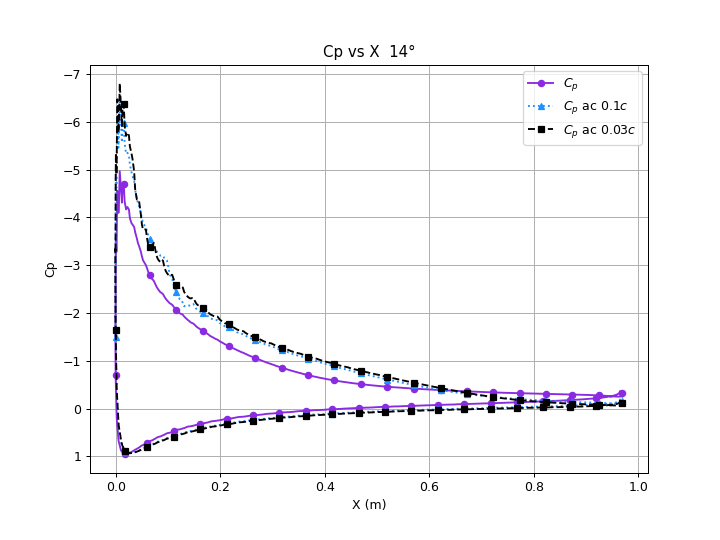
\includegraphics[width=0.75\textwidth]{Cpx_rans_14}    
    \caption{Distribución de coeficientes de presión.}         
  \label{fig:Cpx_rans_14}                          
\end{figure}


\begin{figure}[ht!]
\centering
\begin{subfigure}{0.5\textwidth}
  \centering
  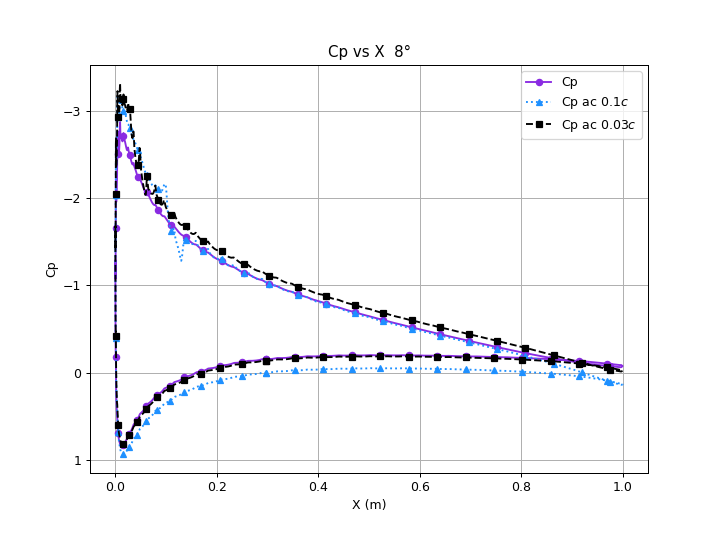
\includegraphics[width=1.0\textwidth]{Cpx_rans_8}
  \caption{Distribución de Cp para $\alpha=8^\circ$.}
  \label{fig:Cpx_rans_8}
\end{subfigure}%
\begin{subfigure}{0.5\textwidth}
  \centering
  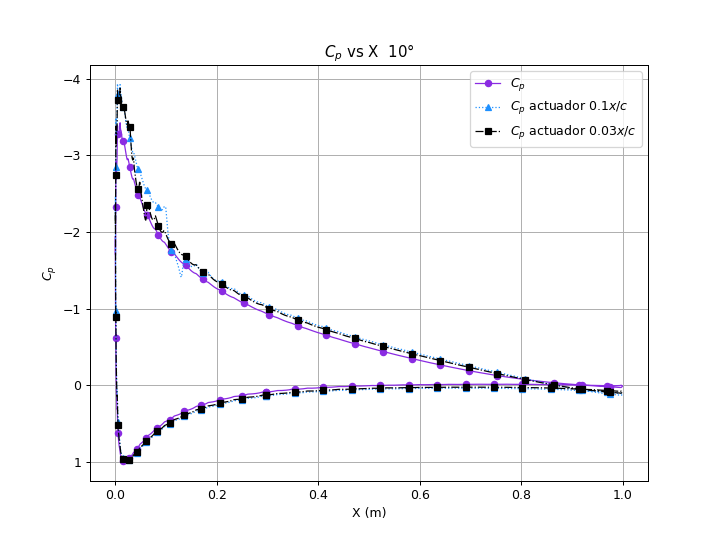
\includegraphics[width=1.0\textwidth]{Cpx_rans_10}
  \caption{Distribución de Cp para $\alpha=10^\circ$.}
  \label{fig:Cpx_rans_10}
\end{subfigure}
\caption{Distribución de presión sobre la superficie del perfil.}
\label{fig:Cpx_rans_a2}
\end{figure}    

\clearpage
\subsection{Arboles de directorios}

Es posible crear arboles de directorios:

\dirtree{%
.1 icoFoam.
.2 Make.
.3 files.
.3 options.
.2 createFields.H.
.2 icoFoam.C.
}

\section{Acrónimos}


Se pueden definir acrónimos usando el comando \verb'\ac' del paquete acro: \ac{rans}, \ac{les}, \ac{dns}

